\documentclass[11pt]{beamer}
\usetheme{Madrid}
\usepackage[utf8]{inputenc}
\usepackage{listings}
\usepackage{tikz}
\usepackage{tkz-euclide}
\usepackage{amsmath}
\usepackage{amsfonts}
\usepackage{amssymb}
\usepackage{graphicx}
\lstset{
%language=C,
frame=single, 
breaklines=true,
columns=fullflexible
}
\setbeamercovered{transparent} 
\setbeamertemplate{navigation symbols}{} 
%\logo{} 

%\date{} 
%\subject{} 


\title{ASSIGNMENT 1}
\author{by Mohit Singh}
\institute{IIEST, Shibpur} 
\centering
\date{21 May 2020}

\begin{document}

\maketitle
\begin{frame}{PROBLEM}
\begin{block}{Exercise 8.1, Q36}
The side AB and BC and median AM of one triangle ABC are respectively equal to sides PQ and QR and median PN of triangle PQR. Show that:
\newline
\newline
{1)$\triangle  ABM  \cong   \triangle  PQN $}
\newline
{2) $\triangle  ABC  \cong   \triangle  PQR $}
\end{block}

\end{frame}

\begin{frame}[containsverbatim]{CODES}
Download the python code from
\begin{lstlisting}
./codes/triangle_python.py
\end{lstlisting}
and latex code from
\begin{lstlisting}
./fig/triangle_fig.tex
\end{lstlisting}
\end{frame}

\begin{frame}{FIGURES}
\begin{figure}
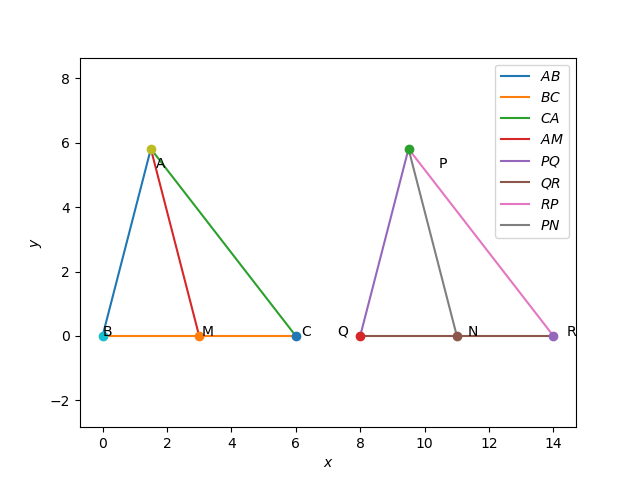
\includegraphics[scale=0.5]{Figure_1.png}
\caption{$\triangle ABC$ and $\triangle PQR$ using Python}
\end{figure}
\end{frame}

\begin{frame}{FIGURES}
\begin{figure}
\resizebox{10cm}{!}{%\documentclass{article}
%\usepackage[utf8]{inputenc}
%\usepackage{tikz}
%\usepackage{tkz-euclide}
%\begin{document}

\begin{tikzpicture}
[scale=1,>=stealth,point/.style={draw,circle,fill = black,inner sep=0.5pt},]

%Triangle sides
\def\a{6}
\def\b{5}
\def\c{6}
 
%Coordinates of A
\def\p{47/12}
%\def\p{4}
\def\q{{sqrt(\c^2-\p^2)}}

%Labeling points
\node (A) at (\p,\q)[point,label=above right:$A$] {};
\node (B) at (0, 0)[point,label=below left:$B$] {};
\node (C) at (\a, 0)[point,label=below right:$C$] {};

%Foot of perpendicular

\node (M) at (\a/2,0)[point,label=above right:$D$] {};

%Drawing triangle ABC
\draw (A) -- node[left] {$\textrm{c}$} (B) -- node[below] {$\textrm{a}$} (C) -- node[above,xshift=2mm] {$\textrm{b}$} (A);

%Drawing median AM
\draw (A) -- node[left] {$\textrm{}$}(M);

%Drawing and marking angles
\tkzMarkAngle[fill=orange!40,size=0.5cm,mark=](C,B,A)
\tkzLabelAngle[pos=-0.9](A,B,C){$\alpha$}

\end{tikzpicture}

\begin{tikzpicture}
[scale=1,>=stealth,point/.style={draw,circle,fill = black,inner sep=0.5pt},]

%Triangle sides
\def\p{6}
\def\q{5}
\def\r{6}
 
%Coordinates of P
\def\x{47/12}
%\def\p{4}
\def\z{{sqrt(\r^2-\x^2)}}

%Labeling points
\node (P) at (\x,\z)[point,label=above right:$P$] {};
\node (Q) at (0, 0)[point,label=below left:$Q$] {};
\node (R) at (\p, 0)[point,label=below right:$R$] {};

%Foot of median

\node (N) at (\p/2,0)[point,label=above right:$N$] {};

%Drawing triangle PQR
\draw (P) -- node[left] {$\textrm{r}$} (Q) -- node[below] {$\textrm{p}$} (R) -- node[above,xshift=2mm] {$\textrm{q}$} (P);

%Drawing median PN
\draw (P) -- node[left] {$\textrm{}$}(N);

%Drawing and marking angles
\tkzMarkAngle[fill=orange!40,size=0.5cm,mark=](R,Q,P)
\tkzLabelAngle[pos=-0.9](P,Q,R){$\theta$}

\end{tikzpicture}
%\end{document}
}
%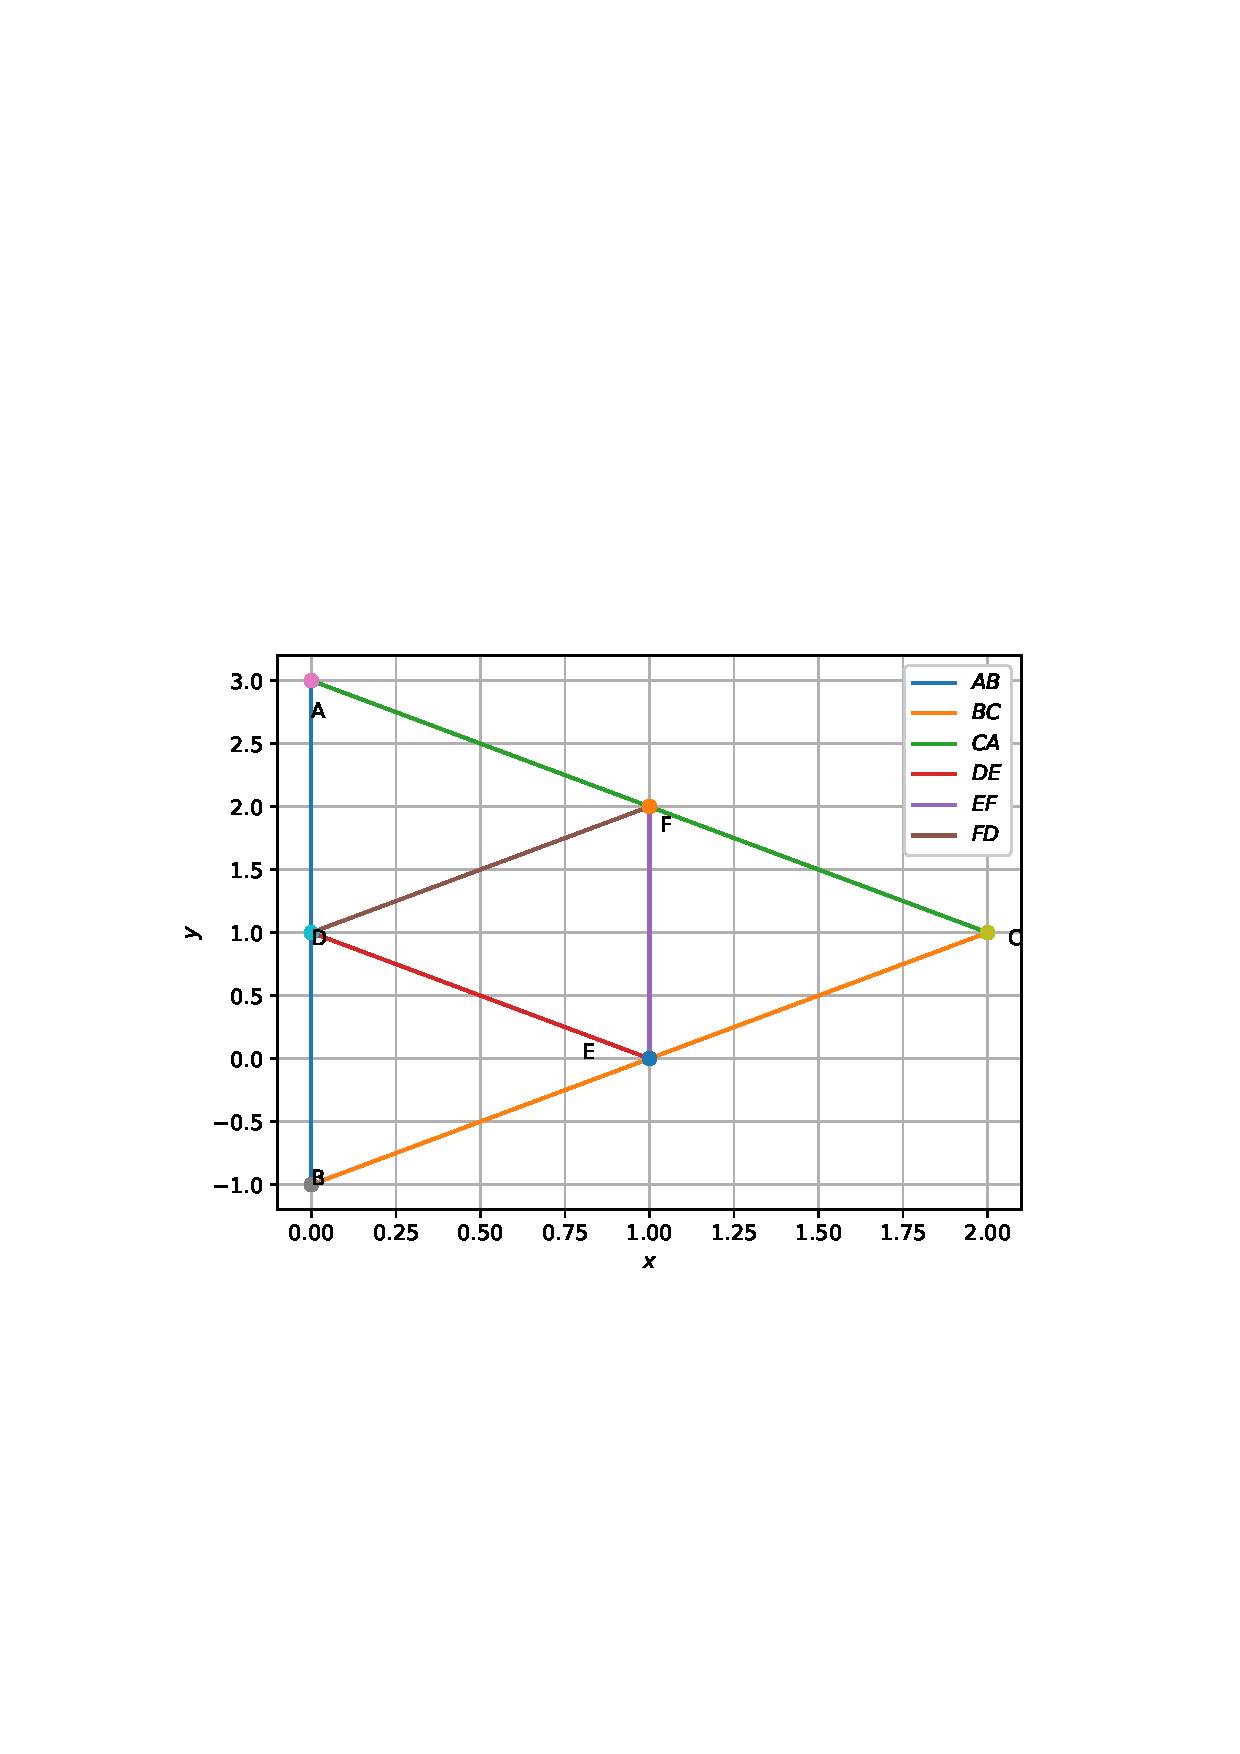
\includegraphics[scale=0.5]{triangle.tex}
\caption{$\triangle ABC$ and $\triangle PQR$ using Latex}
\end{figure}
%! Missing \endgroup inserted.
\end{frame}

\begin{frame}{SOLUTION}
    \begin{flushleft}
       
        1) In triangle ABM and triangle PQN
        \newline
        \newline
        AB = PQ  (Given)
        \newline
        AM = PN  (Given)
        \newline
        Since BC = QR and M , N are midpoints of BC and QR respectively, 
        \newline
        BM = QN 
        \newline 
        Therefore by SSS congruence rule, $\triangle  ABM  \cong   \triangle  PQN$ 
        \newline
        \newline
        This implies that $\angle ABM = \angle PQN$    ........(i)

    \end{flushleft}
 

\end{frame}

\begin{frame}{SOLUTION}

\begin{flushleft}

        2) In triangle ABC and triangle PQR
        \newline
        \newline
        AB = PQ  (Given)
        \newline
        $\angle ABC = \angle PQR$ [From (i)]
        \newline
         BC = QR  (Given) 
        \newline 
        \newline
        Therefore by SAS congruence rule, $\triangle  ABC  \cong   \triangle  PQR$ 
        

\end{flushleft}
    
\end{frame}


\begin{frame}
\huge{\centerline{The End}}
\end{frame}

\end{document}
